\documentclass[border=10pt]{standalone}
\usepackage{pgfplots}
\pgfplotsset{compat=1.18}
\usepgfplotslibrary{fillbetween}
\begin{document}
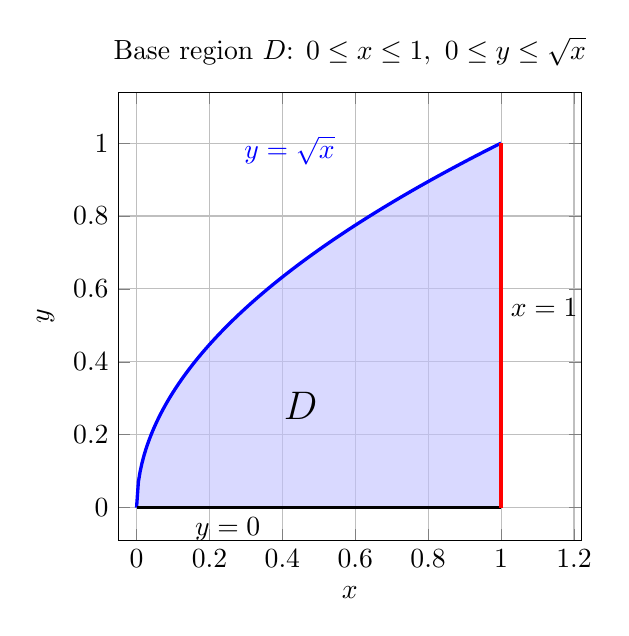
\begin{tikzpicture}
\begin{axis}[
    axis equal image,
    xmin=-0.05,xmax=1.22,ymin=-0.09,ymax=1.14,
    xlabel={$x$}, ylabel={$y$},
    title={Base region $D$: $0\le x\le1,\ 0\le y\le\sqrt{x}$},
    grid=both,
    legend pos=north west,
    samples=200,
]
\addplot[name path=A, domain=0:1, blue, very thick] {sqrt(x)};
\addplot[name path=B, domain=0:1, black, thick] {0};
\addplot[blue!25, opacity=0.6] fill between[of=A and B];
\addplot[red, very thick] coordinates {(1,0) (1,1)};
\node[right] at (axis cs:1,0.55) {$x=1$};
\node at (axis cs:0.45,0.28) {\Large $D$};
\node[blue] at (axis cs:0.42,0.98) {$y=\sqrt{x}$};
\node[below] at (axis cs:0.25,0.0) {$y=0$};
\end{axis}
\end{tikzpicture}
\end{document}
